\section{Fonction caractéristique}

Chapter 1 introduced the fonction génératrice
$G_{X}(t) = \expec(t^{X})$ for two things: reading moments off derivatives, and turning the
loi of a sum of independent variables into a product. Both were bought at a price --- $G_{X}$
is defined only for a variable with values in $\mathbb{N}$, and its moment formula needs a
left derivative at $1$ that may be infinite.\\

The \textbf{fonction caractéristique} (\textit{characteristic function}) buys the same two
uses at no price at all: it is defined for every real variable aléatoire, with no integrability
hypothesis and no restriction on the support, because $e^{itX}$ has modulus $1$ and a
bounded complex variable aléatoire always has an espérance. That single fact makes this
chapter the hinge of the second half of the course. It defines $\varphi_{X}$, proves by the
formule d'inversion that it determines the loi, extracts
moments from its derivatives at $0$,
proves that it turns sums of independent variables into products, transposes all of this to
vecteurs aléatoires, and closes with the criterion chapter 7 runs on: the components of a
vecteur aléatoire are independent exactly when the joint fonction caractéristique factorises.
Chapter 8 proves the théorème central limite by computing one limit of fonctions caractéristiques.

\subsection{Définition et premières propriétés}

\begin{definition}[Fonction caractéristique]
La \textbf{fonction caractéristique} d'une variable aléatoire réelle $X$ est la fonction
$\varphi_{X} \colon \reals \to \mathbb{C}$ définie par :
\[
  \forall t \in \reals, \qquad \varphi_{X}(t) = \expec\!\left(e^{itX}\right).
\]
\end{definition}

La fonction caractéristique est donc l'espérance d'une variable aléatoire \emph{complexe}.
En identifiant une variable aléatoire complexe comme un vecteur aléatoire de dimension $2$, on
en définit l'espérance comme le complexe formé des espérances de ses parties réelles et
imaginaires :
\[
  \expec\!\left(e^{itX}\right) = \expec\!\left(\cos(tX)\right) +
  i\,\expec\!\left(\sin(tX)\right).
\]

\begin{remark}
\textbf{No hypothesis is needed for $\varphi_{X}$ to exist.} Whatever the loi of $X$ ---
heavy-tailed, without espérance, without variance --- la fonction caractéristique est
toujours bien définie, both of the two real integrals above converging absolutely, car :
\[
  \forall t \in \reals, \qquad \expec\!\left(\left|\cos(tX)\right|\right) \leq 1 \quad
  \text{and} \quad \expec\!\left(\left|\sin(tX)\right|\right) \leq 1,
\]
a bounded mesurable function of $X$ being integrable under any mesure de probabilité.
Equivalently, $\left|e^{itX}\right| = 1$ pointwise. This is the contrast with the fonction
génératrice of chapter 1, which needs $X$ to take values in $\mathbb{N}$ and whose derivatives
at $1$ may be infinite. The fonction caractéristique of the loi de Cauchy, which has no
espérance at all, appears later in this chapter and is perfectly well behaved.
\end{remark}

\begin{prop}[Premières propriétés]
La fonction caractéristique est continue, telle que $\varphi_{X}(0) = 1$ et
\[
  \forall t \in \reals, \qquad \left|\varphi_{X}(t)\right| \leq 1.
\]
\end{prop}

\begin{remark}
Three separate facts, each one line. For each fixed $x$, les fonctions $t
\mapsto \cos(tx)$ et $t \mapsto \sin(tx)$ étant continues en $t$ et bornées --- both are
dominated by the constant $1$, which is integrable because $\prob$ is finite ---, la
continuité est une conséquence du théorème de continuité sous le signe somme of chapter 3.
The value at $0$ is
$\expec(e^{0}) = \expec(1) = 1$. L'inégalité vient de chapter 4's probabilistic triangle
inequality, read on
$\mathbb{C} = \reals^{2}$ with the modulus as the norm, so that
$|\expec(Z)| \leq \expec(|Z|)$ for an integrable complex $Z$ --- applied to $Z = e^{itX}$:
$\left|\varphi_{X}(t)\right| \leq \expec\!\left(\left|e^{itX}\right|\right) = 1$. So the
curve $t \mapsto \varphi_{X}(t)$ lives in the closed unit disc of $\mathbb{C}$ and passes
through the point $1$ at $t = 0$.
\end{remark}

\begin{remark}
The converse is false. Toute fonction satisfaisant les conditions de la proposition ---
continuous, equal to $1$ at $0$ and bounded by $1$ in modulus --- n'est \emph{pas}
nécessairement la fonction caractéristique d'une variable aléatoire réelle. Il faut en plus
s'assurer que cette fonction soit définie positive, and with that hypothesis the
characterisation is exact. C'est le \textbf{théorème de Bochner} (\textit{Bochner's theorem}).
It is used below only to assert that a given function \emph{is} a fonction caractéristique
without exhibiting the loi.
\end{remark}

Two structural remarks follow from the definition alone. First, replacing $X$ by $-X$
conjugates:
\[
  \forall t \in \reals, \qquad \varphi_{-X}(t) = \expec\!\left(e^{-itX}\right) =
  \bar{\varphi_{X}(t)}.
\]
Hence la fonction caractéristique d'une variable aléatoire $X$ dont la loi est
\textbf{symétrique} (\textit{symmetric}), au sens où $\prob_{X} = \prob_{-X}$, est à valeurs
réelles, since then $\varphi_{X} = \bar{\varphi_{X}}$ --- a quick sanity check on any
computation. Second, when $X$ has a densité, $\varphi_{X}$ is a Fourier transform.

\begin{remark}[Transformée de Fourier]
Si $X$ a une densité $f_{X}$ par rapport à la mesure de Lebesgue $\lambda$, alors sa
fonction caractéristique est la transformée de Fourier de cette densité: by the
théorème de transfert of chapter 3,
$\varphi_{X}(t) = \int e^{itx} f_{X}(x)\,dx$ for every $t \in \reals$, which is the Fourier
transform of $f_{X}$ in the convention that puts no constant in front and no minus sign in
the exponent. Everything here is therefore Fourier analysis in probabilistic clothing, and
the formule d'inversion of the next subsection is the Fourier inversion theorem.
\end{remark}

\subsubsection{Les cinq lois discrètes}

The five discrete lois of chapter 1 all have fonctions caractéristiques that come straight
from the definition and the théorème de transfert, which for a discrete loi reduces the
espérance to a sum:
\[
  \varphi_{X}(t) = \sum_{k \in S} \prob(X = k)\, e^{itk}, \qquad S \text{ the support.}
\]
The computations below are the ones chapter 9's table states.

\begin{example}[Loi de Bernoulli]
For $X \sim \mathcal{B}(p)$ with $p \in [0,1]$, the support is $\{0,1\}$ and
\[
  \forall t \in \reals, \qquad \varphi_{X}(t) = (1-p)\,e^{i \cdot 0 \cdot t} + p\,e^{i \cdot
  1 \cdot t} = 1 - p + p\,e^{it}.
\]
At $t = 0$ this is $1$, as it must be, and its modulus is at most $1$ because it is a convex
combination of two points of the unit circle.
\end{example}

\begin{example}[Loi binomiale]
For $X \sim \mathcal{B}(n,p)$ with $n \in \mathbb{N}$ and $p \in [0,1]$, the binomial
theorem gives
\[
  \varphi_{X}(t) = \sum_{k=0}^{n} \binom{n}{k} p^{k}(1-p)^{n-k} e^{itk} = \sum_{k=0}^{n}
  \binom{n}{k} \left(p e^{it}\right)^{k}(1-p)^{n-k} = \left(1 - p + p\,e^{it}\right)^{n}.
\]
The answer is the Bernoulli fonction caractéristique raised to the power $n$, which is no
accident: it is the product rule for sums of independent variables, proved below, applied to
$n$ independent Bernoulli variables.
\end{example}

\begin{example}[Loi de Poisson]
For $X \sim \mathcal{P}(\lambda)$ with $\lambda > 0$, the support is $\mathbb{N}$ and the
exponential series sums the result in closed form:
\[
  \varphi_{X}(t) = \sum_{k \geq 0} e^{-\lambda}\frac{\lambda^{k}}{k!}\,e^{itk} =
  e^{-\lambda} \sum_{k \geq 0} \frac{\left(\lambda e^{it}\right)^{k}}{k!} = e^{-\lambda}
  e^{\lambda e^{it}} = \exp\!\left(\lambda\left(e^{it} - 1\right)\right).
\]
The series converges absolutely for every $t$ because $\left|\lambda e^{it}\right| =
\lambda$.
\end{example}

\begin{example}[Loi géométrique]
For $X \sim \mathcal{G}(p)$ with $p \in\, ]0,1]$, the support is $\mathbb{N}^{*}$ and
$\prob(X = k) = (1-p)^{k-1}p$. Factoring out one term and summing the geometric series,
\[
  \varphi_{X}(t) = \sum_{k \geq 1} (1-p)^{k-1} p\, e^{itk} = p\,e^{it} \sum_{j \geq 0}
  \left((1-p)e^{it}\right)^{j} = \frac{p\,e^{it}}{1 - (1-p)e^{it}}.
\]
The geometric series converges because $\left|(1-p)e^{it}\right| = 1 - p < 1$ for $p \in\,
]0,1[$; for $p = 1$ the variable is the constant $1$ and the formula degenerates correctly
to $\varphi_{X}(t) = e^{it}$.
\end{example}

\begin{example}[Loi uniforme discrète]
For $X \sim \mathcal{U}(1,\dots,n)$ with $n \in \mathbb{N}^{*}$, each of the $n$ points
carries mass $1/n$ and the sum is a finite geometric one. For $t \notin 2\pi\zee$,
\[
  \varphi_{X}(t) = \frac{1}{n}\sum_{k=1}^{n} e^{itk} = \frac{1}{n}\, e^{it}\,\frac{e^{int} -
  1}{e^{it} - 1} = e^{i(n+1)t/2}\,\frac{\sin(nt/2)}{n \sin(t/2)},
\]
the second form obtained by factoring $e^{int/2}$ out of the numerator and $e^{it/2}$ out of
the denominator. For $t \in 2\pi\zee$ every term of the sum is $1$ and $\varphi_{X}(t) = 1$;
the excluded points are exactly the zeros of the denominator, and the function extends
continuously across them.
\end{example}

\subsubsection{Les quatre lois à densité}

For a loi with a densité the théorème de transfert turns the espérance into an intégrale de
Lebesgue, and the four lois of the densité table are computed below. Three have elementary
closed forms; the fourth deliberately does not, and saying so is part of the run.

\begin{example}[Loi exponentielle]
For $X \sim \mathcal{E}(\lambda)$ with $\lambda > 0$, the densité is $\lambda e^{-\lambda
x}\indic_{\reals_{+}}(x)$ and
\[
  \varphi_{X}(t) = \int_{0}^{+\infty} e^{itx}\,\lambda e^{-\lambda x}\,dx = \lambda
  \int_{0}^{+\infty} e^{-(\lambda - it)x}\,dx = \frac{\lambda}{\lambda - it}.
\]
The improper integral converges because $\left|e^{-(\lambda - it)x}\right| = e^{-\lambda x}$
with $\lambda > 0$, and $\lambda - it$ never vanishes for the same reason, so no case
distinction is needed. The loi is not symétrique and the answer is genuinely complex.
\end{example}

\begin{example}[Loi Gamma]
For $X \sim \Gamma(a,\lambda)$ with $a, \lambda > 0$, the densité is
$\frac{\lambda^{a}}{\Gamma(a)}x^{a-1}e^{-\lambda x}\indic_{\reals_{+}}(x)$. The computation
is the exponential one with a normalisation trick: multiply and divide so that what remains
under the integral is again a gamma densité, this time with parameter $\lambda - it$ in
place of $\lambda$.
\[
  \varphi_{X}(t) = \int_{0}^{+\infty}
  e^{itx}\,\frac{\lambda^{a}}{\Gamma(a)}x^{a-1}e^{-\lambda x}\,dx = \int_{0}^{+\infty}
  \frac{\lambda^{a}}{\Gamma(a)}x^{a-1}e^{-(\lambda-it)x}\,dx
\]
\[
  \phantom{\varphi_{X}(t)} = \left(\frac{\lambda}{\lambda - it}\right)^{a}
  \int_{0}^{+\infty} \frac{(\lambda - it)^{a}}{\Gamma(a)}x^{a-1}e^{-(\lambda-it)x}\,dx =
  \left(\frac{\lambda}{\lambda - it}\right)^{a},
\]
the last integral being $1$ because its integrand is the analytic continuation of a gamma
densité and $\Re(\lambda - it) = \lambda > 0$. The power is the principal branch, continuous
in $t$ and equal to $1$ at $t = 0$. Setting $a = 1$ recovers the loi exponentielle, as it
must.
\end{example}

\begin{example}[Loi uniforme continue]
For $X \sim \mathcal{U}([a,b])$ with $a < b$, the densité is
$\frac{1}{b-a}\indic_{[a,b]}(x)$ and, for $t \neq 0$,
\[
  \varphi_{X}(t) = \int_{a}^{b} e^{itx}\,\frac{dx}{b-a} = \frac{e^{itb} -
  e^{ita}}{it\,(b-a)},
\]
while $\varphi_{X}(0) = 1$. The case distinction at $t = 0$ is genuine --- the written
expression is $0/0$ there --- and the extension is by continuity. Two specialisations recur.
On $[-1,1]$ the loi is symétrique and the answer collapses to the real function
\[
  \varphi_{X}(t) = \frac{e^{it} - e^{-it}}{2it} = \frac{\sin t}{t}, \qquad t \neq 0,
\]
the \textbf{cardinal sine}; and on $[0,1]$ it is $\left(e^{it}-1\right)/(it)$, which the
moment subsection expands.
\end{example}

\begin{example}[Loi Beta]
For $X \sim \mathcal{B}(a,b)$ with $a, b > 0$, the densité is
$\frac{1}{B(a,b)}x^{a-1}(1-x)^{b-1}\indic_{[0,1]}(x)$ and there is no closed form in
elementary functions. What there is instead is a convergent series, obtained by expanding
$e^{itx}$ and integrating term by term --- legitimate by convergence dominée, the partial
sums being dominated by $e^{|t|}$ times the densité on the bounded support $[0,1]$. Since
$\expec(X^{k}) = B(a+k,b)/B(a,b) = \prod_{r=0}^{k-1}\frac{a+r}{a+b+r}$,
\[
  \varphi_{X}(t) = \sum_{k \geq 0} \frac{(it)^{k}}{k!}\,\expec\!\left(X^{k}\right) = \sum_{k
  \geq 0} \left(\prod_{r=0}^{k-1}\frac{a+r}{a+b+r}\right)\frac{(it)^{k}}{k!},
\]
which is the confluent hypergeometric function $M(a,\,a+b,\,it)$. Every moment exists
because the support is bounded, so the series is the Taylor series at $0$ in the strongest
sense and the moment theorem below applies at every order. Chapter 9's table records the
series and not a closed form, because there is none to record.
\end{example}

\begin{example}[Loi normale centrée réduite, par une équation différentielle]
For $X \sim \mathcal{N}(0,1)$ the direct integral is not elementary, and the way in is en
dérivant sous le signe somme, puis en intégrant par parties. Write
\[
  \varphi_{X}(t) = \int e^{itx}\,\frac{1}{\sqrt{2\pi}}\,e^{-x^{2}/2}\,dx.
\]
The partial derivative in $t$ of the integrand is
$ixe^{itx}\frac{1}{\sqrt{2\pi}}e^{-x^{2}/2}$, dominated in modulus by
$|x|\frac{1}{\sqrt{2\pi}}e^{-x^{2}/2}$, which is integrable and does not depend on $t$; the
théorème de dérivabilité sous le signe somme of chapter 3 therefore applies and gives
\[
  \varphi_{X}'(t) = i\int x\,e^{itx}\,\frac{1}{\sqrt{2\pi}}\,e^{-x^{2}/2}\,dx = -i\int
  e^{itx}\,\frac{1}{\sqrt{2\pi}}\,\frac{d}{dx}\!\left(e^{-x^{2}/2}\right)dx = i\int
  (it)\,e^{itx}\,\frac{1}{\sqrt{2\pi}}\,e^{-x^{2}/2}\,dx = -t\,\varphi_{X}(t),
\]
using $x e^{-x^{2}/2} = -\frac{d}{dx}e^{-x^{2}/2}$ and then an integration by parts in
which the bracketed term vanishes at
$\pm\infty$. So $\varphi_{X}$ vérifie l'équation différentielle $\varphi_{X}'(t) =
-t\,\varphi_{X}(t)$, which is linear, with $\varphi_{X}(0) = 1$, and since the loi is
symétrique, $\varphi_{X}$ est une fonction réelle. That Cauchy problem has the unique solution
\[
  \forall t \in \reals, \qquad \varphi_{X}(t) = e^{-t^{2}/2}.
\]
The loi normale centrée réduite is thus its own Fourier transform up to normalisation --- the
fact chapter 7 builds vecteurs gaussiens on and chapter 8's théorème central limite identifies
as its limit.
\end{example}

\begin{figure}[ht]
\centering
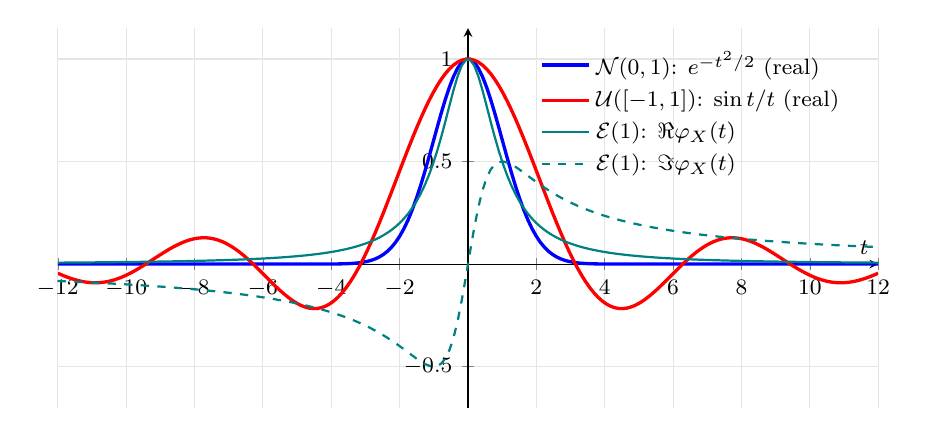
\begin{tikzpicture}
\begin{axis}[
  width=12cm, height=6.4cm, xlabel={$t$}, xmin=-12, xmax=12, ymin=-0.7, ymax=1.15,
  axis lines=middle, samples=200, domain=-12:12, grid=major, grid style={gray!20},
  legend pos=north east, legend cell align=left,
  legend style={font=\footnotesize, draw=none, fill=none},
  tick label style={font=\footnotesize}, label style={font=\footnotesize},
]
\addplot[very thick, blue]  {exp(-x^2/2)};
\addlegendentry{$\mathcal{N}(0,1)$: $e^{-t^{2}/2}$ (real)}
\addplot[very thick, red]   {sin(deg(x))/x};
\addlegendentry{$\mathcal{U}([-1,1])$: $\sin t / t$ (real)}
\addplot[thick, teal]       {1/(1+x^2)};
\addlegendentry{$\mathcal{E}(1)$: $\Re \varphi_{X}(t)$}
\addplot[thick, teal, dashed] {x/(1+x^2)};
\addlegendentry{$\mathcal{E}(1)$: $\Im \varphi_{X}(t)$}
\end{axis}
\end{tikzpicture}
\caption{Fonctions caractéristiques of three lois on a shared axis. The two
lois symétriques give real-valued curves; the exponential, which is not symétrique, needs both
a real and an imaginary part. All four curves pass through or below the level $1$, and the
two real ones take the value $1$ at $t = 0$.}
\end{figure}

\begin{figure}[ht]
\centering
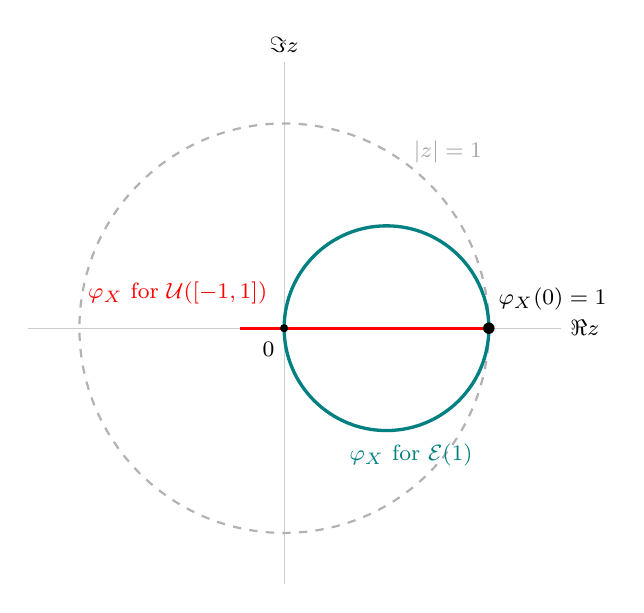
\begin{tikzpicture}[scale=2.6]
\draw[gray!40] (-1.25,0) -- (1.35,0) node[right, font=\footnotesize, black] {$\Re z$};
\draw[gray!40] (0,-1.25) -- (0,1.3) node[above, font=\footnotesize, black] {$\Im z$};
\draw[thick, gray!60, dashed] (0,0) circle (1);
\node[gray!70, font=\footnotesize] at (0.80,0.86) {$|z| = 1$};
\draw[very thick, teal] (0.5,0) circle (0.5);
\node[teal, font=\footnotesize] at (0.62,-0.62) {$\varphi_{X}$ for $\mathcal{E}(1)$};
\draw[very thick, red] (-0.2172,0) -- (1,0);
\node[red, font=\footnotesize] at (-0.52,0.17) {$\varphi_{X}$ for $\mathcal{U}([-1,1])$};
\fill (1,0) circle (0.028);
\node[font=\footnotesize, anchor=south west] at (1.0,0.04) {$\varphi_{X}(0) = 1$};
\fill (0,0) circle (0.02);
\node[font=\footnotesize, anchor=north east] at (0,-0.02) {$0$};
\end{tikzpicture}
\caption{The bound $|\varphi_{X}(t)| \leq 1 = \varphi_{X}(0)$, drawn in the
complex plane. Whatever the loi, the trajectory $t \mapsto \varphi_{X}(t)$ stays inside the
closed unit disc and touches its boundary at $t = 0$. For $\mathcal{E}(1)$ the trajectory is
exactly the circle of centre $1/2$ and radius $1/2$, tangent to the unit circle at $1$; for
the loi symétrique $\mathcal{U}([-1,1])$ it is a real segment, $\sin t / t$ ranging over
$[-0.2172\ldots,\,1]$.}
\end{figure}

\subsection{Formule d'inversion}

La \textbf{formule d'inversion} (\textit{inversion formula}) permet d'exprimer la loi d'une variable aléatoire réelle à partir de sa
fonction caractéristique. Avant d'énoncer ce résultat, on montre comment obtenir les atomes de
la loi --- by the same technique, worth seeing first because the whole proof of the formule
d'inversion is that computation with a better kernel.

\begin{prop}[Atomes de la loi]
Soit $X$ une variable aléatoire réelle. Alors,
\[
  \forall x \in \reals, \qquad \prob(X = x) = \lim_{T \to +\infty} \frac{1}{2T}\int_{-T}^{T}
  e^{-itx}\,\varphi_{X}(t)\,dt.
\]
\end{prop}

\begin{remark}
The mechanism is a Dirichlet-kernel computation followed by an exchange of limit,
espérance and integral. On fixe $x$. Pour tout $y \neq x$,
\[
  \frac{1}{2T}\int_{-T}^{T} e^{-itx}e^{ity}\,dt = \frac{1}{2T}\,\frac{e^{iT(y-x)} -
  e^{-iT(y-x)}}{i(y-x)} = \frac{\sin\!\left(T(y-x)\right)}{T(y-x)},
\]
which tends to $0$ as $T \to +\infty$; for $y = x$ the integrand is $1$ and the average is
$1$ for every $T$. En remplaçant $y$ par la variable aléatoire $X$ et en prenant l'espérance,
the limit inside is $\indic_{\{X = x\}}$. On conclut par le théorème de convergence dominée
et le théorème de Fubini, which move the limit and the espérance past the integral. Les
conditions de ces théorèmes sont bien réunies --- both are licensed by the same one-line
bound --- puisque :
\[
  \left|\frac{1}{2T}\int_{-T}^{T} e^{-itx}e^{itX}\,dt\right| \leq
  \frac{1}{2T}\int_{-T}^{T}\left|e^{-itx}e^{itX}\right|dt = 1,
\]
a constant, which is integrable because $\prob$ is a finite mesure.
\end{remark}

\begin{theorem}[Formule d'inversion]
Soit $X$ une variable aléatoire réelle de fonction de répartition $F_{X}$. Alors pour tous
\emph{points de continuité} $a, b$ de $F_{X}$, avec $a < b$,
\[
  F_{X}(b) - F_{X}(a) = \lim_{T \to +\infty} \frac{1}{2\pi}\int_{-T}^{T} \frac{e^{-ita} -
  e^{-itb}}{it}\,\varphi_{X}(t)\,dt.
\]
\end{theorem}

The hypothesis that $a$ and $b$ be continuity points of $F_{X}$ is not decoration. The proof
below produces, for arbitrary $a < b$, the quantity $\prob(a < X < b) + \tfrac{1}{2}\prob(X
= a) + \tfrac{1}{2}\prob(X = b)$, which equals $F_{X}(b) - F_{X}(a)$ as soon as neither
endpoint is an atom. The half weights at the endpoints are the signature of a Dirichlet
kernel and they are exactly what the continuity hypothesis kills.

\begin{proof}
On fixe $a < b$. Pour tout $T > 0$, soit :
\[
  I_{T} = \int_{-T}^{T} \frac{e^{-ita} - e^{-itb}}{it}\,e^{itx}\,dt,
\]
which is well defined: la fonction à intégrer, once extended by continuity, est continue sur
$[-T,T]$ --- near $t = 0$ the numerator vanishes to first order and cancels the $it$ in the
denominator.\\

\textbf{Step 1: reduce $I_{T}$ to Dirichlet integrals.} Splitting the range at $0$ and
substituting $t \mapsto -t$ on the negative half,
\[
  I_{T} = \int_{0}^{T} \frac{e^{-ita} - e^{-itb}}{it}\,e^{itx}\,dt + \int_{0}^{T}
  \frac{e^{ita} - e^{itb}}{-it}\,e^{-itx}\,dt
\]
\[
  \phantom{I_{T}} = \int_{0}^{T} \frac{e^{it(x-a)} - e^{-it(x-a)}}{it}\,dt - \int_{0}^{T}
  \frac{e^{it(x-b)} - e^{-it(x-b)}}{it}\,dt
\]
\[
  \phantom{I_{T}} = 2\left(\int_{0}^{T} \frac{\sin\!\left(t(x-a)\right)}{t}\,dt -
  \int_{0}^{T} \frac{\sin\!\left(t(x-b)\right)}{t}\,dt\right) = 2\left(\int_{0}^{T(x-a)}
  \frac{\sin u}{u}\,du - \int_{0}^{T(x-b)} \frac{\sin u}{u}\,du\right),
\]
the last equality by the changement de variable $u = t(x-a)$ in the first integral and $u =
t(x-b)$ in the second, valid with the sign conventions because $u \mapsto \sin u / u$ is
even.\\

\textbf{Step 2: take $T \to +\infty$ using the Dirichlet integral.} The classical Dirichlet
integral --- quoted here as an intégrale de Riemann impropre, chapter 3 recording its value $\pi$
over the whole line together with the warning that it is improper-Riemann and not
Lebesgue --- states
\[
  \int_{0}^{+\infty} \frac{\sin u}{u}\,du = \frac{\pi}{2}.
\]
Applying it to each of the two terms of Step 1, according to the signs of $x - a$ and $x -
b$, gives
\[
  \lim_{T \to +\infty} \frac{1}{2\pi}\int_{-T}^{T} \frac{e^{-ita} -
  e^{-itb}}{it}\,e^{itx}\,dt =
  \begin{cases} 1           & \text{if } x \in\, ]a,b[,\\[2pt]
  \tfrac{1}{2} & \text{if } x \in \{a,b\},\\[2pt] 0           & \text{otherwise.}
  \end{cases}
\]
En remplaçant $x$ par la variable aléatoire $X$ et en prenant l'espérance of this limit,
\[
  \expec\!\left(\lim_{T \to +\infty} \frac{1}{2\pi}\int_{-T}^{T} \frac{e^{-ita} -
  e^{-itb}}{it}\,e^{itX}\,dt\right) = \prob(a < X < b) + \tfrac{1}{2}\prob(X = a) +
  \tfrac{1}{2}\prob(X = b).
\]

\textbf{Step 3: exchange the limit and the espérance.} Par le théorème de convergence
dominée, the limit comes out of the espérance:
\[
  \lim_{T \to +\infty} \frac{1}{2\pi}\,\expec\!\left(\int_{-T}^{T} \frac{e^{-ita} -
  e^{-itb}}{it}\,e^{itX}\,dt\right) = \prob(a < X < b) + \tfrac{1}{2}\prob(X = a) +
  \tfrac{1}{2}\prob(X = b).
\]
Les conditions d'application du théorème sont bien satisfaites car Step 1 has already bounded
the integral, uniformly in $T$ and in $X$, by a finite constant:
\[
  \forall T \geq 0, \qquad \left|\int_{-T}^{T} \frac{e^{-ita} -
  e^{-itb}}{it}\,e^{itX}\,dt\right| \leq 4 \sup_{s \geq 0} \left|\int_{0}^{s} \frac{\sin
  u}{u}\,du\right| < \infty,
\]
the supremum being finite because $s \mapsto \int_{0}^{s}\sin u / u\,du$ is continuous with
a finite limit at $+\infty$. A constant is integrable under a mesure de probabilité, so
convergence dominée applies.\\

\textbf{Step 4: exchange the espérance and the $dt$ integral.} Le théorème de Fubini donne :
\[
  \expec\!\left(\int_{-T}^{T} \frac{e^{-ita} - e^{-itb}}{it}\,e^{itX}\,dt\right) =
  \int_{-T}^{T} \frac{e^{-ita} - e^{-itb}}{it}\,\expec\!\left(e^{itX}\right)dt =
  \int_{-T}^{T} \frac{e^{-ita} - e^{-itb}}{it}\,\varphi_{X}(t)\,dt.
\]
Fubini needs the mesure produit to be $\sigma$-finie --- it is, $\prob$ being finite and the
mesure de Lebesgue on the bounded interval $[-T,T]$ being finite too --- and needs the integrand
to be integrable for the mesure produit. À nouveau, les conditions d'application du théorème
sont bien satisfaites car, for every real $x$,
\[
  \left|\frac{e^{-ita} - e^{-itb}}{it}\,e^{itx}\right| = \left|\frac{e^{it(b-a)/2} -
  e^{-it(b-a)/2}}{t}\right| = \left|\frac{2\sin\!\left(t(b-a)/2\right)}{t}\right| \leq b -
  a,
\]
de sorte que
\[
  \expec\!\left(\left|\int_{-T}^{T} \frac{e^{-ita} -
  e^{-itb}}{it}\,e^{itX}\,dt\right|\right) \leq 2T\,(b-a) < \infty.
\]

\textbf{Step 5: conclude.} Finalement, combining Steps 3 and 4,
\[
  \lim_{T \to +\infty} \frac{1}{2\pi}\int_{-T}^{T} \frac{e^{-ita} -
  e^{-itb}}{it}\,\varphi_{X}(t)\,dt = \prob(a < X < b) + \tfrac{1}{2}\prob(X = a) +
  \tfrac{1}{2}\prob(X = b).
\]
Lorsque $a$ et $b$ sont des points de continuité de $F_{X}$, the two atoms vanish and the
right-hand side is $\prob(a < X \leq b) = F_{X}(b) - F_{X}(a)$: on obtient le résultat
annoncé.
\end{proof}

\begin{remark}
Each exchange in the proof is justified by its own explicit bound --- $4\sup_{s}
\left|\int_{0}^{s}\sin u/u\right|$ for convergence dominée, $b-a$ for Fubini --- and that is
the shape of every serious computation here: write the kernel, bound it by something
integrable that does not depend on the parameter being sent to a limit, then exchange. The
bound $\left|\sin(cs)/s\right| \leq |c|$ is used twice and is worth remembering separately.
\end{remark}

\begin{corollary}[Caractérisation de la loi]
Pour toutes variables aléatoires réelles $X, Y$, on a
\[
  \prob_{X} = \prob_{Y} \iff \varphi_{X} = \varphi_{Y}.
\]
\end{corollary}

\begin{remark}
La condition nécessaire est immédiate, par le théorème de transfert: equal lois give equal
espérances of every bounded mesurable function, in particular of $x \mapsto e^{itx}$. The
converse is the formule d'inversion plus one countability argument. Soit $A$ et $B$ les
ensembles des atomes of the two lois; ces ensembles étant au plus dénombrables, c'est
également le cas de $A \union B$, whose complement is therefore dense and unbounded below.
Pour tout $b \notin A \union B$, la formule d'inversion donne $F_{X}(b) -
F_{X}(a) = F_{Y}(b) - F_{Y}(a)$ for every $a \notin A \union B$, and letting $a \to -\infty$
en dehors de $A \union B$ yields $F_{X}(b) = F_{Y}(b)$; par ailleurs, pour tout
$b \in A \union B$, right continuity gives $F_{X}(b) = \lim_{a \downarrow b} F_{X}(a)$, the
limit again taken en dehors de $A \union B$, and the same for $Y$. On a finalement
$F_{X} = F_{Y}$, si bien que $\prob_{X} = \prob_{Y}$.
\end{remark}

La fonction caractéristique porte bien son nom, au sens où elle caractérise la loi, and this
is what every later use rests on: to identify the loi of a complicated variable aléatoire,
compute its fonction caractéristique and recognise the answer. Chapters 7 and 8 both identify
a loi that way.

\begin{corollary}[Formule d'inversion pour une loi à densité]
Soit $X$ une variable aléatoire réelle dont la fonction caractéristique est \emph{intégrable
sur $\reals$}. Alors $X$ a pour densité la fonction :
\[
  \forall x \in \reals, \qquad f_{X}(x) = \frac{1}{2\pi}\int e^{-itx}\,\varphi_{X}(t)\,dt.
\]
\end{corollary}

\begin{remark}
The integrability of $\varphi_{X}$ over the whole line is the hypothesis that makes this
work and it cannot be weakened to the boundedness the first proposition of the chapter gives
for free. It does two jobs. First it kills the atoms --- la loi n'a pas d'atome --- by the
atom formula,
\[
  \left|\frac{1}{2T}\int_{-T}^{T}e^{-itx}\varphi_{X}(t)\,dt\right| \leq
  \frac{1}{2T}\int_{-T}^{T}\left|\varphi_{X}(t)\right|dt \leq \frac{1}{2T}\int
  \left|\varphi_{X}(t)\right|dt \xrightarrow[T \to +\infty]{} 0,
\]
so $\prob(X = x) = 0$ for every $x$ and the half-weight terms of the formule d'inversion drop.
Second it licenses a Fubini and a convergence dominée in the computation
\[
  \prob(a < X < b) = \lim_{T\to+\infty}
  \frac{1}{2\pi}\int_{-T}^{T}\left(\int_{a}^{b}e^{-itx}dx\right)\varphi_{X}(t)\,dt =
  \int_{a}^{b}\left(\frac{1}{2\pi}\int e^{-itx}\varphi_{X}(t)\,dt\right)dx,
\]
which exhibits the bracketed function as a densité of $X$ on every interval, hence --- the
intervals generating $\mathcal{B}(\reals)$ --- as a densité. Note the asymmetry of the two
formulas: $\varphi_{X}$ is an integral of $e^{itx}$ against the loi, and $f_{X}$ an integral
of $e^{-itx}$ against $\varphi_{X}$, divided by $2\pi$.
\end{remark}

\begin{example}[Recovering the Cauchy densité from its fonction caractéristique]
Let $\varphi_{X}(t) = e^{-|t|}$. By the théorème de Bochner, cette fonction est la fonction
caractéristique d'une certaine variable aléatoire réelle $X$ --- it is continuous, equal to $1$
at $0$ and bounded by $1$, and it is définie positive, which is the extra hypothesis the
théorème de Bochner asks for and which is not checked here --- and it is integrable on
$\reals$, with $\int e^{-|t|}dt = 2$. The formule d'inversion pour une loi à densité therefore
applies and gives
\[
  f_{X}(x) = \frac{1}{2\pi}\int e^{-itx}e^{-|t|}\,dt =
  \frac{1}{2\pi}\left(\int_{-\infty}^{0} e^{-itx}e^{t}\,dt + \int_{0}^{+\infty}
  e^{-itx}e^{-t}\,dt\right)
\]
\[
  \phantom{f_{X}(x)} = \frac{1}{2\pi}\left(\frac{1}{1 - ix} + \frac{1}{1 + ix}\right) =
  \frac{1}{2\pi}\cdot\frac{2}{1 + x^{2}} = \frac{1}{\pi\left(1 + x^{2}\right)}.
\]
Il s'agit de la loi de Cauchy. The example is instructive twice
over: it is a loi produced from a fonction caractéristique rather than the other way round,
and it is the standard counter-example of the next subsection, having no espérance at all.
\end{example}

\subsection{Calcul de moments}

The second use of the fonction caractéristique is the one chapter 1 had for the fonction
génératrice: derivatives at a point return moments. Here the point is $0$ rather than $1^{-}$,
and the derivatives are two-sided.

\begin{definition}[Moment]
Soit $k$ un entier non nul. On appelle \textbf{moment d'ordre $k$} (\textit{moment of order
$k$}) d'une variable aléatoire réelle $X$ la valeur $\expec(X^{k})$, lorsqu'elle est bien
définie. On dit que $X$ \textbf{admet un moment d'ordre $k$} si cette valeur est finie.
\end{definition}

\begin{lemma}
Une variable aléatoire $X$ qui admet un moment d'ordre $k$ admet des moments jusqu'à l'ordre
$k$ (au moins).
\end{lemma}

\begin{remark}
One line of algebra. On a pour tout $j = 1,\dots,k$,
\[
  |X|^{j} \leq \max\!\left(|X|^{k},\,1\right) \leq |X|^{k} + 1,
\]
the first inequality because $u \mapsto u^{j}$ is below $\max(u^{k},1)$ on $\reals_{+}$ for
$j \leq k$. En appliquant l'espérance, $\expec(|X|^{j})$ is finite whenever $\expec(|X|^{k})$
is, and $\expec(1) = 1 < \infty$ because $\prob$ is a mesure de probabilité. The lemma is what
lets the moment theorem differentiate $k$ times rather than only once.
\end{remark}

\begin{theorem}[Calcul de moments]
Si la variable aléatoire $X$ \emph{admet un moment d'ordre $k$}, alors sa fonction
caractéristique $\varphi_{X}$ est $k$ fois dérivable en $0$ et
\[
  \varphi_{X}^{(k)}(0) = i^{k}\,\expec\!\left(X^{k}\right).
\]
Réciproquement, si la fonction caractéristique $\varphi_{X}$ est $k$ fois dérivable en $0$,
\emph{avec $k$ pair}, alors la variable aléatoire $X$ admet des moments jusqu'à l'ordre $k$
et ceux-ci sont donnés par la formule précédente.
\end{theorem}

Both hypotheses are load-bearing and neither may be dropped. The direct implication needs
$X$ to admit a moment d'ordre $k$ --- without it there is nothing to dominate the $k$-th
derivative of the integrand and the conclusion itself fails --- $\varphi_{X}$ need not
even be differentiable at $0$ --- as the loi de Cauchy shows below. The converse needs $k$
\emph{even} because the proof does: the sign identity
$-\varphi_{X}''(0) = \left|\varphi_{X}''(0)\right|$, and the induction step behind it, rest
on the positivity of $X^{2p}\left(1 - \cos(tX)\right)$. The caveat stated separately below ---
that $\varphi_{X}$ being of class $C^{1}$ does not make $X$ integrable --- is the same
restriction at the first order.

\begin{remark}
\textbf{The direct implication.} Pour tout $x$ réel, on a :
\[
  \frac{\partial^{k}}{\partial t^{k}}\,e^{itx} = i^{k}x^{k}e^{itx}, \qquad\text{hence}\qquad
  \left|\frac{\partial^{k}}{\partial t^{k}}\,e^{itX}\right| = |X|^{k},
\]
a dominating function that does not depend on $t$ and is integrable exactly because $X$
admet un moment d'ordre $k$. The lemma above supplies the same for every intermediate order
$j \leq k$, so \textbf{le théorème de dérivabilité sous le signe somme} of chapter 3 may
be applied $k$ times in succession --- that theorem is the dependency, and it is what the
hypothesis on the moment is there to feed. Evaluating at $t = 0$, on en déduit que :
\[
  \varphi_{X}^{(k)}(0) = \frac{\partial^{k}}{\partial
  t^{k}}\expec\!\left(e^{itX}\right)\Big|_{t=0} = i^{k}\,\expec\!\left(X^{k}\right).
\]
\end{remark}

\begin{remark}
\textbf{The converse.} A Taylor expansion at $0$ turned into an inequality by the lemme de
Fatou, run at $k = 2$ and then by induction on $p$ for $k = 2p$. Two-fold
differentiability at $0$ and the identity
$\varphi_{X}(t) + \varphi_{X}(-t) = 2\,\expec\!\left(\cos(tX)\right)$ give
\[
  \lim_{t \to 0} \frac{2}{t^{2}}\,\expec\!\left(1 - \cos(tX)\right) = -\varphi_{X}''(0) =
  \left|\varphi_{X}''(0)\right|,
\]
la dernière égalité venant du fait que le terme de gauche est positif, $1 - \cos \geq 0$ ---
which is exactly where the parity of $k$ enters. Along any $t_{n} \to 0$ the integrand tends
to $X^{2}$, so, par le lemme de Fatou, $\expec(X^{2})$ is bounded by
$\left|\varphi_{X}''(0)\right| < \infty$. The
induction step repeats this with $\varphi_{X}^{(2p)}$ in place of $\varphi_{X}$, using the
induction hypothesis $\varphi_{X}^{(2p)}(0) = (-1)^{p}\expec(X^{2p})$ and differentiating
the same cosine identity $2p$ times under the integral sign, to bound
$\expec(X^{2p+2})$ by $\left|\varphi_{X}^{(2p+2)}(0)\right| < \infty$.
\end{remark}

\begin{remark}
A caveat that is easy to lose: il n'est \textbf{pas} suffisant que la fonction
caractéristique $\varphi_{X}$ soit de classe $C^{1}$ pour que la variable aléatoire $X$ soit
intégrable. Une condition suffisante est que $\varphi_{X}$ soit de classe $C^{2}$. This is the
same parity phenomenon as in the theorem, stated for the weakest case: one derivative buys
nothing, two buy a first and a second moment.
\end{remark}

In practice the theorem is almost never applied by differentiating $k$ times. It is applied
by expanding $\varphi_{X}$ in a Taylor series at $0$ and reading the coefficients: once
$\varphi_{X}$ is known to be $k$ times differentiable at $0$, the theorem fixes its Taylor
coefficients as the $i^{j}\expec(X^{j})/j!$, so matching any expansion against
$\sum_{j \leq k} i^{j}\expec(X^{j})\,t^{j}/j! + o(t^{k})$ reads the moments off. The
expansion alone is weaker than the differentiability the theorem asks for, so it is a way of
applying the theorem and not a restatement of it. Three examples show the pattern, and one
shows the failure.

\begin{example}[Moments de la loi exponentielle]
For $X \sim \mathcal{E}(\lambda)$ the fonction caractéristique $\varphi_{X}(t) =
\lambda/(\lambda - it)$ expands as a geometric series in $it/\lambda$:
\[
  \varphi_{X}(t) = \frac{1}{1 - it/\lambda} = 1 + \frac{it}{\lambda} +
  \left(\frac{it}{\lambda}\right)^{2} + o(t^{2}) = 1 + \frac{it}{\lambda} -
  \frac{t^{2}}{\lambda^{2}} + o(t^{2}).
\]
Matching against $1 + i\expec(X)t - \expec(X^{2})t^{2}/2 + o(t^{2})$ gives
\[
  \expec(X) = \frac{1}{\lambda}, \qquad \expec\!\left(X^{2}\right) = \frac{2}{\lambda^{2}},
  \qquad \Var(X) = \frac{2}{\lambda^{2}} - \frac{1}{\lambda^{2}} = \frac{1}{\lambda^{2}}.
\]
\end{example}

\begin{example}[{Moments de la loi uniforme sur $[0,1]$}]
For $X \sim \mathcal{U}([0,1])$, $\varphi_{X}(t) = \left(e^{it}-1\right)/(it)$ for $t \neq
0$. Comme $e^{it} = 1 + it - t^{2}/2 - it^{3}/6 + o(t^{3})$, on obtient, dividing by $it$ :
\[
  \varphi_{X}(t) = 1 + \frac{it}{2} - \frac{t^{2}}{6} + o(t^{2}),
\]
on en déduit
\[
  \expec(X) = \frac{1}{2}, \qquad \expec\!\left(X^{2}\right) = \frac{1}{3}, \qquad \Var(X) =
  \frac{1}{3} - \frac{1}{4} = \frac{1}{12}.
\]
\end{example}

\begin{example}[Moments de la loi Gamma]
For $X \sim \Gamma(a,\lambda)$, $\varphi_{X}(t) = (1 - it/\lambda)^{-a}$, and the binomial
series $(1-u)^{-a} = 1 + au + a(a+1)u^{2}/2 + o(u^{2})$ with $u = it/\lambda$ gives
\[
  \varphi_{X}(t) = 1 + \frac{ia\,t}{\lambda} - \frac{a(a+1)}{2}\,\frac{t^{2}}{\lambda^{2}} +
  o(t^{2}),
\]
so that
\[
  \expec(X) = \frac{a}{\lambda}, \qquad \expec\!\left(X^{2}\right) =
  \frac{a(a+1)}{\lambda^{2}}, \qquad \Var(X) = \frac{a(a+1) - a^{2}}{\lambda^{2}} =
  \frac{a}{\lambda^{2}}.
\]
Setting $a = 1$ recovers the exponential line above, as a check.
\end{example}

\begin{example}[Les quatre premiers moments de la loi normale centrée réduite]
For $X \sim \mathcal{N}(0,1)$, $\varphi_{X}(t) = e^{-t^{2}/2}$, and expanding the
exponential to two terms,
\[
  \varphi_{X}(t) = 1 - \frac{t^{2}}{2} + \frac{t^{4}}{8} + o\!\left(t^{4}\right).
\]
The odd powers are absent, which is the symmetry of the loi reappearing. Matching
coefficients against $\sum_{j \leq 4} i^{j}\expec(X^{j})t^{j}/j!$ gives
\[
  \expec(X) = 0, \qquad \expec\!\left(X^{2}\right) = 1, \qquad \expec\!\left(X^{3}\right) =
  0, \qquad \expec\!\left(X^{4}\right) = 3.
\]
The fourth moment being $3$ rather than $1$ is the value worth memorising, and it is read
straight off the $t^{4}$ coefficient of $e^{-t^{2}/2}$.
\end{example}

\begin{example}[A loi whose fonction caractéristique is not differentiable at zero]
La loi de Cauchy n'a pas d'espérance: $\int |x|/(\pi(1+x^{2}))\,dx$ diverges logarithmically.
Its fonction caractéristique is $\varphi_{X}(t) = e^{-|t|}$, which is continuous everywhere,
of modulus at most $1$, equal to $1$ at $0$ --- and cette fonction n'est \emph{pas} dérivable
en $0$, the left and right derivatives being $+1$ and $-1$. The theorem's direct implication
is therefore consistent: a loi with no moment d'ordre $1$ may not have a differentiable
fonction caractéristique at $0$. This is the example to reach for whenever the hypothesis
``$X$ admet un moment d'ordre $k$'' looks removable.
\end{example}

\subsection{Somme de variables aléatoires indépendantes}

The third use --- and the one chapter 8 runs on --- is that the fonction caractéristique converts
the convolution of lois into an ordinary product of functions.

\begin{prop}
Soit $X$ et $Y$ deux variables aléatoires réelles indépendantes. La fonction caractéristique
de leur somme est donnée par :
\[
  \forall t \in \reals, \qquad \varphi_{X+Y}(t) = \varphi_{X}(t)\,\varphi_{Y}(t).
\]
\end{prop}

\begin{proof}
Fix $t \in \reals$. Since $X \indep Y$, the variables aléatoires $e^{itX}$ and $e^{itY}$ are
independent as well, being mesurable functions of $X$ and of $Y$ respectively; both are
bounded, hence integrable, so the product rule for espérances of independent integrable
variables applies:
\[
  \varphi_{X+Y}(t) = \expec\!\left(e^{it(X+Y)}\right) =
  \expec\!\left(e^{itX}\,e^{itY}\right) =
  \expec\!\left(e^{itX}\right)\expec\!\left(e^{itY}\right) = \varphi_{X}(t)\,\varphi_{Y}(t).
\]
\end{proof}

\begin{remark}
One line, and it is worth noticing what does \emph{not} appear in it. There is no
integrability hypothesis on $X$ or $Y$, because $e^{itX}$ and $e^{itY}$ are bounded whatever
the lois; there is no hypothesis of a densité, so the result covers discrete and continuous
lois at once; and there is no convolution integral to compute. Combined with the corollary
that the fonction caractéristique determines the loi, the proposition is a complete method
for finding the loi of a sum of independent variables: multiply, then recognise. By
induction it extends immediately to $n$ independent summands, and for $n$ i.i.d.\ summands
it reads $\varphi_{S_{n}} = \varphi_{X_{1}}^{\,n}$ --- which is the identity the théorème
central limite is proved from in chapter 8.
\end{remark}

\begin{figure}[ht]
\centering
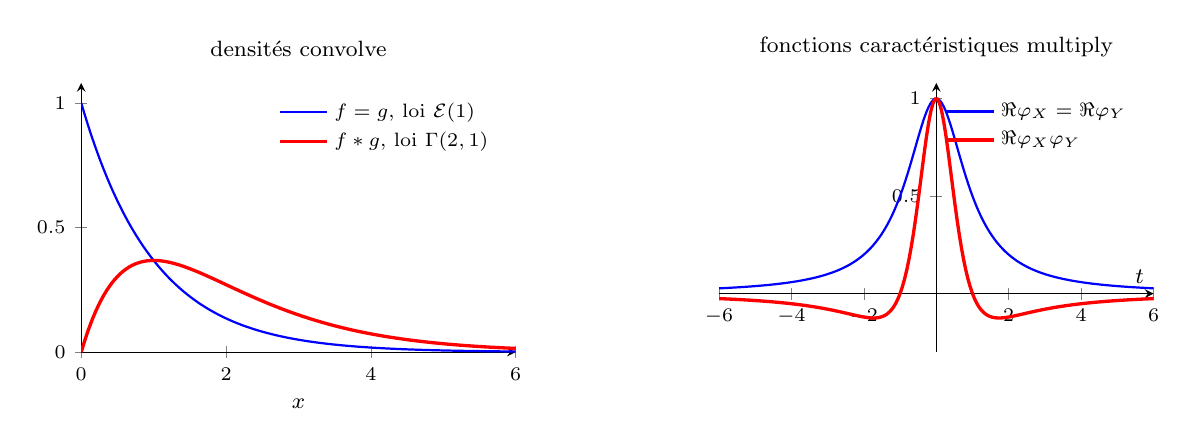
\begin{tikzpicture}
\begin{axis}[
  name=densities, width=7.1cm, height=5.0cm, xlabel={$x$},
  title={\footnotesize densités convolve}, title style={font=\footnotesize},
  xmin=0, xmax=6, ymin=0, ymax=1.08, axis lines=left, samples=120, domain=0:6,
  legend pos=north east, legend cell align=left,
  legend style={font=\scriptsize, draw=none, fill=none},
  tick label style={font=\scriptsize}, label style={font=\footnotesize},
]
\addplot[thick, blue] {exp(-x)};
\addlegendentry{$f = g$, loi $\mathcal{E}(1)$}
\addplot[very thick, red] {x*exp(-x)};
\addlegendentry{$f * g$, loi $\Gamma(2,1)$}
\end{axis}
\begin{axis}[
  at={(8.1cm,0cm)}, anchor=south west, width=7.1cm, height=5.0cm, xlabel={$t$},
  title={\footnotesize fonctions caractéristiques multiply}, title style={font=\footnotesize},
  xmin=-6, xmax=6, ymin=-0.3, ymax=1.08, axis lines=middle, samples=200, domain=-6:6,
  legend pos=north east, legend cell align=left,
  legend style={font=\scriptsize, draw=none, fill=none},
  tick label style={font=\scriptsize}, label style={font=\footnotesize},
]
\addplot[thick, blue] {1/(1+x^2)};
\addlegendentry{$\Re \varphi_{X} = \Re \varphi_{Y}$}
\addplot[very thick, red] {(1-x^2)/((1+x^2)^2)};
\addlegendentry{$\Re \varphi_{X}\varphi_{Y}$}
\end{axis}
\end{tikzpicture}
\caption{The product rule, drawn. On the left, two $\mathcal{E}(1)$ densités
and their convolution, the $\Gamma(2,1)$ densité $x e^{-x}$; on the right, the real parts of
the corresponding fonctions caractéristiques, the product $\left(1/(1-it)\right)^{2}$ having
real part $(1-t^{2})/(1+t^{2})^{2}$. The convolution on the left costs an integral; the
product on the right costs a multiplication.}
\end{figure}

\begin{example}[A normal variable with general parameters]
Soit $Z \sim \mathcal{N}(0,1)$. La variable aléatoire $X = \sigma Z + \mu$ suit une loi normale
$\mathcal{N}(\mu,\sigma^{2})$. An affine changement de variable inside the espérance gives
\[
  \forall t \in \reals, \qquad \varphi_{X}(t) = \expec\!\left(e^{it(\sigma Z + \mu)}\right)
  = e^{i\mu t}\,\varphi_{Z}(\sigma t) = e^{i\mu t}\,e^{-\sigma^{2}t^{2}/2}.
\]
The two operations used --- $\varphi_{aX+b}(t) = e^{ibt}\varphi_{X}(at)$ --- are worth
isolating, since they are needed again in chapter 8 to normalise a sum.
\end{example}

\begin{example}[The sum of two independent normal variables is normal]
Let $X \sim \mathcal{N}(\mu_{1},\sigma_{1}^{2})$ and $Y \sim
\mathcal{N}(\mu_{2},\sigma_{2}^{2})$ be independent. Multiplying the fonctions
caractéristiques of the previous example,
\[
  \varphi_{X+Y}(t) = e^{i\mu_{1}t}e^{-\sigma_{1}^{2}t^{2}/2}\,
  e^{i\mu_{2}t}e^{-\sigma_{2}^{2}t^{2}/2} = e^{i(\mu_{1}+\mu_{2})t}\,
  e^{-\left(\sigma_{1}^{2}+\sigma_{2}^{2}\right)t^{2}/2},
\]
which is the fonction caractéristique of
$\mathcal{N}(\mu_{1}+\mu_{2},\,\sigma_{1}^{2}+\sigma_{2}^{2})$. Since the fonction
caractéristique determines the loi, the sum follows that loi: la somme de deux variables
aléatoires indépendantes suivant des lois normales suit une loi normale, d'espérance la somme
des espérances et de variance la somme des variances. The indépendance hypothesis
is essential --- without it only the means add.
\end{example}

\begin{example}[A sum of independent exponential variables is a gamma variable]
Soit $X_{1},\dots,X_{n}$ des variables aléatoires i.i.d.\ de loi $\mathcal{E}(\lambda)$ et
$S = X_{1} + \dots + X_{n}$ leur somme. The product rule and the exponential computation give
\[
  \varphi_{S}(t) = \varphi_{X_{1}}(t)\cdots\varphi_{X_{n}}(t) =
  \left(\varphi_{X_{1}}(t)\right)^{n} = \left(\frac{\lambda}{\lambda - it}\right)^{n},
\]
which is la fonction caractéristique d'une loi $\Gamma(n,\lambda)$. Hence $S \sim
\Gamma(n,\lambda)$. Computing the same convolution directly would mean $n-1$ nested
integrals.
\end{example}

\begin{example}[The gamma family is stable in its first parameter]
Soit $X \sim \Gamma(a,\lambda)$ et $Y \sim \Gamma(b,\lambda)$ indépendantes, with the
\emph{same} second parameter $\lambda$. Then
\[
  \forall t \in \reals, \qquad \varphi_{X+Y}(t) = \left(\frac{\lambda}{\lambda -
  it}\right)^{a} \left(\frac{\lambda}{\lambda - it}\right)^{b} =
  \left(\frac{\lambda}{\lambda - it}\right)^{a+b},
\]
so $X + Y \sim \Gamma(a+b,\lambda)$. The equality of the two $\lambda$'s is what makes the
exponents add; with different rate parameters the product is not of gamma form and the sum
is not a gamma variable.
\end{example}

\begin{example}[The loi du $\chi^{2}$ as a loi Gamma]
For $Z \sim \mathcal{N}(0,1)$, combining the two exponents and rescaling the Gaussian
integral --- legitimate for a complex parameter of positive real part --- gives
\[
  \varphi_{Z^{2}}(t) = \expec\!\left(e^{itZ^{2}}\right) = \int
  e^{itz^{2}}\frac{1}{\sqrt{2\pi}}e^{-z^{2}/2}\,dz = \int e^{-\frac{1}{2}(1 -
  2it)z^{2}}\frac{1}{\sqrt{2\pi}}\,dz = \frac{1}{\sqrt{1 - 2it}},
\]
which is $\left(\tfrac{1}{2}/(\tfrac{1}{2} - it)\right)^{1/2}$, la fonction caractéristique
d'une loi $\Gamma(\tfrac{1}{2},\tfrac{1}{2})$. By definition, la \textbf{loi du $\chi^{2}$ à
$n$ degrés de liberté} (\textit{chi-squared distribution with $n$ degrees of freedom}) est une
loi Gamma $\Gamma(\tfrac{n}{2},\tfrac{1}{2})$, so the previous example gives at once that la
somme des carrés de $n$ variables aléatoires normales centrées réduites indépendantes suit une
loi du $\chi^{2}$ à $n$ degrés de liberté, and that la somme de deux variables indépendantes de
lois du $\chi^{2}$ à $n$ et $m$ degrés de liberté follows a loi du $\chi^{2}$ à $n + m$
degrés de liberté.
\end{example}

\begin{example}[A geometric number of exponential summands]
Soit $X_{1}, X_{2}, \dots$ une suite de variables aléatoires i.i.d.\ de loi $\mathcal{E}(\lambda)$,
et $N$ une variable aléatoire de loi géométrique $\mathcal{G}(p)$ de paramètre $p \in\, ]0,1[$,
indépendante de cette suite. On note $S = \sum_{i=1}^{N} X_{i}$, a sum with a \emph{random}
number of terms. Conditioning on $N$ and using the
previous computation for a fixed number of summands,
\[
  \varphi_{S}(t) = \sum_{n \geq 1} \prob(N = n)\, \expec\!\left(e^{itS} \mid N = n\right) =
  \sum_{n \geq 1} (1-p)^{n-1}p\left(\frac{\lambda}{\lambda - it}\right)^{n} =
  \frac{p\lambda}{p\lambda - it},
\]
the last step being the geometric sum $\sum_{n \geq 1}(1-p)^{n-1}p\,z^{n} = pz/(1-(1-p)z)$
with $z = \lambda/(\lambda - it)$. So $S \sim \mathcal{E}(p\lambda)$: a geometric number of
independent exponential waiting times is again an exponential waiting time, with the rate
thinned by $p$. The conditioning step is the discrete espérance conditionnelle of chapter 1,
and the interchange of the sum and the espérance is convergence dominée, the partial
sums being bounded by $1$.
\end{example}

\begin{example}[The loi de Cauchy is stable under averaging]
Soit $X_{1},\dots,X_{n}$ des variables aléatoires i.i.d.\ suivant la loi de Cauchy, so
$\varphi_{X_{1}}(t) = e^{-|t|}$. The fonction caractéristique of the arithmetic mean is
\[
  \varphi_{\frac{1}{n}(X_{1}+\dots+X_{n})}(t) =
  \varphi_{X_{1}+\dots+X_{n}}\!\left(\frac{t}{n}\right) =
  \left(\varphi_{X_{1}}\!\left(\frac{t}{n}\right)\right)^{n} = \left(e^{-|t|/n}\right)^{n} =
  e^{-|t|},
\]
so la moyenne arithmétique of $n$ i.i.d.\ Cauchy variables suit une loi de Cauchy --- the same
one, whatever $n$.
Averaging buys nothing, and neither does averaging in the other sense: the inverse of a
Cauchy variable is again a Cauchy variable, so the $1/X_{i}$ are i.i.d.\ with the loi de
Cauchy, their arithmetic mean is Cauchy by the computation just made, and la moyenne
harmonique $n/(1/X_{1}+\dots+1/X_{n})$, being the inverse of that arithmetic mean, suit
également une loi de Cauchy. This
is the standard illustration that the loi forte des grands nombres and
the théorème central limite of chapter 8 genuinely need their moment hypotheses, which the
loi de Cauchy fails at the first order.
\end{example}

\begin{remark}[The parallel with the fonction génératrice of chapter 1]
The two transforms of the course have the same two uses and differ in one respect only.
\begin{itemize}
  \item \textbf{Moments by differentiation.} $G_{X}$ gives factorial moments
    from left derivatives at $1$, when those are finite, and $\varphi_{X}$ gives ordinary
    moments from two-sided derivatives at $0$, when the moment exists:
    \[
      \expec\!\left(X(X-1)\cdots(X-k+1)\right) = G_{X}^{(k)}\!\left(1^{-}\right), \qquad
      \varphi_{X}^{(k)}(0) = i^{k}\,\expec\!\left(X^{k}\right).
    \]
  \item \textbf{Products for sums of independents.} $G_{X+Y} = G_{X}G_{Y}$ and
    $\varphi_{X+Y} = \varphi_{X}\varphi_{Y}$, proved by exactly the same line: the
    exponential turns a sum into a product and indépendance splits the espérance.
  \item \textbf{The difference.} $G_{X}(t) = \expec(t^{X})$ requires $X$ to
    take values in $\mathbb{N}$ and requires $|t| \leq 1$ for the series to converge, and
    even then its derivative at $1$ may be infinite. $\varphi_{X}$ requires nothing at all:
    it is defined for every real variable aléatoire and every real $t$, because
    $\left|e^{itX}\right| = 1$. That is the whole of the advantage, and it is why the
    fonction caractéristique and not the fonction génératrice is the tool of chapters 7 and 8.
\end{itemize}
Both transforms characterise the loi --- $G_{X}$ through $\prob(X = k) = G_{X}^{(k)}(0)/k!$,
$\varphi_{X}$ through the formule d'inversion --- so the choice between them is a matter of
which is easier to compute, and for an $\mathbb{N}$-valued variable that is often $G_{X}$.
\end{remark}

\subsection{Cas des vecteurs aléatoires}

Les résultats précédents se généralisent à des vecteurs aléatoires réels. The scalar results
are deliberately restated below rather than generalised in place, in compressed form: the
statements come first and the remark that follows says which of them are word-for-word
transpositions and which are genuinely different.

\begin{definition}[Fonction caractéristique d'un vecteur aléatoire]
La \textbf{fonction caractéristique} d'un vecteur aléatoire réel $X$ de dimension $n$ est la
fonction $\varphi_{X} \colon \reals^{n} \to \mathbb{C}$ définie par :
\[
  \forall t \in \reals^{n}, \qquad \varphi_{X}(t) =
  \expec\!\left(e^{i\,t^{T}X}\right),
\]
where $t^{T}X = t_{1}X_{1} + \dots + t_{n}X_{n}$.
\end{definition}

As in dimension $1$, la fonction caractéristique est continue, telle que $\varphi_{X}(0) =
1$ et
\[
  \forall t \in \reals^{n}, \qquad \left|\varphi_{X}(t)\right| \leq 1,
\]
for the same three reasons: continuité sous le signe somme with the constant $1$ as
dominating function, the value of the integrand at $t = 0$, and the modulus inequality
applied to a variable of modulus $1$.

\begin{theorem}[Formule d'inversion pour un vecteur aléatoire]
Soit $X$ un vecteur aléatoire réel de fonction de répartition $F_{X}$. Alors pour tous points
de continuité $a, b$ de $F_{X}$, avec $a < b$ \emph{composante par composante},
\[
  F_{X}(b) - F_{X}(a) = \lim_{T_{1} \to +\infty}\ \dots \lim_{T_{n} \to +\infty}
  \frac{1}{(2\pi)^{n}}\int_{-T_{1}}^{T_{1}}\!\!\dots\int_{-T_{n}}^{T_{n}}
  \prod_{j=1}^{n}\frac{e^{-it_{j}a_{j}} - e^{-it_{j}b_{j}}}{it_{j}}\, \varphi_{X}(t)\,dt.
\]
\end{theorem}

\begin{corollary}[Caractérisation de la loi]
Pour tous vecteurs aléatoires réels $X, Y$, on a
\[
  \prob_{X} = \prob_{Y} \iff \varphi_{X} = \varphi_{Y}.
\]
\end{corollary}

\begin{corollary}[Formule d'inversion pour une loi à densité]
Soit $X$ un vecteur aléatoire réel dont la fonction caractéristique est \emph{intégrable sur
$\reals^{n}$}. Alors $X$ a pour densité la fonction :
\[
  \forall x \in \reals^{n}, \qquad f_{X}(x) = \frac{1}{(2\pi)^{n}}\int
  e^{-i\,t^{T}x}\,\varphi_{X}(t)\,dt.
\]
\end{corollary}

\begin{definition}[Moment d'un vecteur aléatoire]
Soit $k$ un entier non nul. On appelle \textbf{moment d'ordre $k$} d'un vecteur aléatoire
réel $X$ le \emph{vecteur} $\expec(X^{k})$, lorsqu'il est bien défini. On dit que $X$ admet
un moment d'ordre $k$ si ce vecteur est fini.
\end{definition}

\begin{lemma}
Soit $X$ un vecteur aléatoire réel qui admet un moment d'ordre $k$. Alors pour tous entiers
naturels $j_{1},\dots,j_{n}$ \emph{de somme inférieure ou égale à $k$},
\[
  \expec\!\left(\left|X_{1}^{j_{1}} \dots X_{n}^{j_{n}}\right|\right) < \infty.
\]
\end{lemma}

\begin{remark}
The same algebraic line as in dimension $1$, with a maximum over the components in place of
a maximum over the orders:
\[
  \left|X_{1}^{j_{1}} \dots X_{n}^{j_{n}}\right| \leq
  \max\!\left(|X_{1}|^{k},\dots,|X_{n}|^{k},\,1\right) \leq |X_{1}|^{k} + \dots +
  |X_{n}|^{k} + 1,
\]
and en appliquant l'espérance, on obtient le résultat annoncé, each term on the right being
finite by hypothesis. What the lemma controls is a \emph{mixed} moment, which has no
counterpart in dimension $1$.
\end{remark}

\begin{theorem}[Calcul de moments d'un vecteur aléatoire]
Si le vecteur aléatoire $X$ admet un moment d'ordre $k$, alors sa fonction caractéristique
$\varphi_{X}$ est $k$ fois dérivable en $0$ et pour tous entiers naturels
$j_{1},\dots,j_{n}$ \emph{de somme égale à $k$},
\[
  \frac{\partial^{\,j_{1}} \dots \partial^{\,j_{n}}} {\partial t_{1}^{\,j_{1}} \dots
  \partial t_{n}^{\,j_{n}}}\, \varphi_{X}(0) = i^{k}\,\expec\!\left(X_{1}^{j_{1}} \dots
  X_{n}^{j_{n}}\right).
\]
Réciproquement, si la fonction caractéristique $\varphi_{X}$ est $k$ fois dérivable en $0$,
\emph{avec $k$ pair}, alors les variables aléatoires $X_{1}^{j_{1}} \dots X_{n}^{j_{n}}$ sont
d'espérances finies, données par la formule précédente, pour tous entiers naturels
$j_{1},\dots,j_{n}$ \emph{de somme inférieure ou égale à $k$}.
\end{theorem}

\begin{remark}
La première partie du théorème se prouve exactly as in dimension $1$, differentiating under
the integral sign, with the vector lemma above supplying the dominating function
$\left|X_{1}^{j_{1}}\dots X_{n}^{j_{n}}\right|$ in place of $|X|^{k}$. The converse reduces
to the scalar theorem by a projection: pour tout $j = 1,\dots,n$, la fonction caractéristique
de la variable aléatoire $X_{j}$ est donnée par $\varphi_{X_{j}}(t) = \varphi_{X}(t e_{j})$
pour tout $t \in \reals$, où $e_{j}$ désigne le vecteur unitaire sur la composante $j$. Cette
fonction caractéristique étant $k$ fois dérivable en $0$, avec $k$ pair, the scalar theorem gives
$X_{j}$ a moment d'ordre $k$; le vecteur aléatoire $X$ admet donc un moment d'ordre $k$, and
the direct implication finishes.
\end{remark}

\begin{remark}[Which of these are verbatim transpositions, and which are not]
Worth separating, because reading the six statements as a block hides the two that carry new
content.
\begin{itemize}
  \item \textbf{Verbatim transpositions}, with $t^{T}x$ in place of
    $tx$ and $\reals^{n}$ in place of $\reals$: the definition of $\varphi_{X}$, the
    continuity and the bounds $\varphi_{X}(0) = 1$ and $\left|\varphi_{X}\right| \leq 1$,
    and the corollary that the fonction caractéristique characterises the loi. Nothing in
    their proofs changes.
  \item \textbf{Transpositions that change shape.} The formule d'inversion
    becomes an \emph{iterated} limit, one $T_{j}$ per coordinate, over a product of $n$
    scalar kernels and with $(2\pi)^{n}$ in the denominator; its hypothesis is that $a < b$
    hold componentwise, which is strictly stronger than $a < b$ for vectors read any other
    way. The formule d'inversion pour une loi à densité keeps the same shape but with
    $(2\pi)^{n}$ and the scalar product in the exponent, and its hypothesis is integrability
    over the whole of $\reals^{n}$.
  \item \textbf{Genuinely different statements.} The lemma is about
    \emph{mixed} moments $\expec\left(\left|X_{1}^{j_{1}}\dots X_{n}^{j_{n}}\right|\right)$
    with $j_{1}+\dots+j_{n} \leq k$, where the scalar lemma was about lower-order moments
    $\expec(|X|^{j})$ with $j \leq k$; and the moment theorem returns \emph{mixed partial}
    derivatives, one formula for each multi-index of total order $k$, where the scalar
    theorem returned one number per order. The converse also changes method, going through
    the projections $\varphi_{X_{j}}(t) = \varphi_{X}(te_{j})$ rather than repeating the
    Fatou argument in $n$ dimensions.
\end{itemize}
The product rule for sums of independent \emph{vectors} holds too, by the same one-line
proof, and is used in chapter 7 to add independent vecteurs gaussiens.
\end{remark}

\subsection{Caractérisation de l'indépendance}

The last result of the chapter is the one chapter 7 is built on. It says that indépendance
of the components of a vecteur aléatoire is not merely implied by a factorisation of the joint
fonction caractéristique --- it is equivalent to it.

\begin{prop}[Caractérisation de l'indépendance]
Soit $X$ un vecteur aléatoire de dimension $n$. Les composantes $X_{1},\dots,X_{n}$ du vecteur
$X$ sont indépendantes si et seulement si
\[
  \forall t \in \reals^{n}, \qquad \varphi_{X}(t) = \varphi_{X_{1}}(t_{1}) \dots
  \varphi_{X_{n}}(t_{n}).
\]
\end{prop}

\begin{remark}
\textbf{La condition nécessaire} est immédiate: if the components are independent then so are
the bounded variables $e^{it_{1}X_{1}},\dots,e^{it_{n}X_{n}}$, and the espérance of their
product splits,
\[
  \varphi_{X}(t) = \expec\!\left(e^{i\,t^{T}X}\right) =
  \expec\!\left(e^{it_{1}X_{1}}\right)\dots\expec\!\left(e^{it_{n}X_{n}}\right) =
  \varphi_{X_{1}}(t_{1})\dots\varphi_{X_{n}}(t_{n}).
\]
\textbf{The sufficient condition} is the interesting direction and it is a one-trick
argument: build a comparison vector and appeal to uniqueness. On considère un vecteur $Y$
dont les composantes sont indépendantes, de mêmes lois marginales que le vecteur $X$ --- such a
$Y$ exists, on a product space, by the mesure produit construction of chapter 3. By the
direction just proved,
\[
  \forall t \in \reals^{n}, \qquad \varphi_{Y}(t) =
  \varphi_{Y_{1}}(t_{1})\dots\varphi_{Y_{n}}(t_{n}) =
  \varphi_{X_{1}}(t_{1})\dots\varphi_{X_{n}}(t_{n}) = \varphi_{X}(t),
\]
the middle equality because $Y_{j}$ and $X_{j}$ have the same loi and hence the same
fonction caractéristique, and the last by hypothesis. The vector corollary that the
fonction caractéristique characterises the loi then gives $\prob_{X} = \prob_{Y}$;
indépendance of the components being a property of the loi jointe alone, the components of
$X$ are independent.
\end{remark}

\begin{remark}
The criterion is a genuine strengthening of what the definition of indépendance gives.
Verifying indépendance from the definition means checking $\prob(X_{1} \in A_{1}, \dots,
X_{n} \in A_{n}) = \prod_{j}\prob(X_{j} \in A_{j})$ for all boréliens $A_{1},\dots,A_{n}$ ---
an uncountable family of conditions on sets. The criterion replaces it by one functional
identity between two explicit functions on $\reals^{n}$, both of which are usually written
down in closed form. Chapter 7 uses it in exactly that way: the fonction caractéristique of a
vecteur gaussien of matrice de covariance $\Gamma$ is $\varphi_{X}(t) =
\exp\!\left(i\,t^{T}\mu - \tfrac{1}{2}t^{T}\Gamma t\right)$, and that
expression factorises into a product of $n$ scalar Gaussian fonctions caractéristiques exactly
when the quadratic form $t^{T}\Gamma t$ has no cross terms, that is, exactly when
$\Gamma$ is diagonal. So for a vecteur gaussien --- and only because the criterion is an
equivalence --- décorrélées components are independent components.
\end{remark}

\begin{conclusion}
The fonction caractéristique $\varphi_{X}(t) = \expec\left(e^{itX}\right)$ exists for every
real variable aléatoire, with no hypothesis, because $\left|e^{itX}\right| = 1$; it is
continuous, equals $1$ at $0$ and is bounded by $1$ in modulus. The formule d'inversion
recovers $F_{X}$ from $\varphi_{X}$ at every pair of continuity points, and therefore
$\varphi_{X}$ determines the loi; when $\varphi_{X}$ is integrable over $\reals$ the same
formula produces a densité. The $k$-th derivative at $0$ returns $i^{k}\expec(X^{k})$ when
the moment d'ordre $k$ exists, and conversely a derivative of even order $k$ at $0$ forces
the moments up to order $k$ to exist. For independent variables $\varphi_{X+Y} =
\varphi_{X}\varphi_{Y}$, which turns convolutions into products. All of this transposes to
vecteurs aléatoires, the formule d'inversion becoming an iterated limit and the moment theorem
returning mixed partial derivatives, and the transposition yields the criterion the next
chapter needs: the components of a vecteur aléatoire are independent exactly when the joint
fonction caractéristique factorises into the product of the marginal ones.
\end{conclusion}
